\documentclass[tikz]{standalone}
\usepackage{amsmath}
\usepackage{times}
\usepackage{txfonts}

\usetikzlibrary{arrows}
\usetikzlibrary{intersections}
\usetikzlibrary{math}
\usetikzlibrary{positioning}
\usetikzlibrary{arrows.meta}
\usetikzlibrary{shapes.misc}
\usetikzlibrary{calc}

\begin{document}
  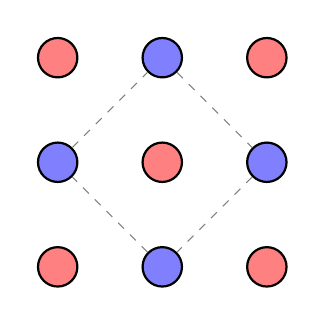
\begin{tikzpicture}[
      >=latex, 
      node distance = 2mm,
      charge/.style = {
        circle, draw = black, thick,
        minimum size = 5mm
      },
      positive/.style = { fill = red!50 },
      negative/.style = { fill = blue!50 },
    ]

    \matrix[nodes = { charge }, row sep = 8mm, column sep = 8mm] {
      \node[positive] {}; & \node[negative] (N) {}; & \node [positive] {}; \\
      \node[negative] (W) {}; & \node[positive] {}; & \node [negative] (E) {}; \\
      \node[positive] {}; & \node[negative] (S) {}; & \node [positive] {}; \\
    };
    \draw[gray, dashed] (W) to (N) to (E) to (S) to (W);
  \end{tikzpicture}
\end{document}
